\documentclass[11pt, a4paper]{article}

% \usepackage[utf8]{utf8}
\usepackage[margin=1in]{geometry}
\usepackage{graphicx}
\usepackage{amsmath, amssymb}
\usepackage{listings}
\usepackage{xcolor}
\usepackage{hyperref}
\usepackage{booktabs}
\usepackage{subcaption}
\usepackage{float}

\definecolor{vscodeBg}{rgb}{0.12, 0.12, 0.12}     
\definecolor{vscodeFg}{rgb}{0.86, 0.86, 0.86}     
\definecolor{vscodeKeyword}{rgb}{0.34, 0.61, 0.84}
\definecolor{vscodeControl}{rgb}{0.77, 0.53, 0.75}
\definecolor{vscodeString}{rgb}{0.81, 0.57, 0.47} 
\definecolor{vscodeComment}{rgb}{0.42, 0.60, 0.33}
\definecolor{vscodeNumber}{rgb}{0.71, 0.80, 0.66} 
\definecolor{vscodeLineNum}{rgb}{0.53, 0.53, 0.53}
\lstdefinestyle{customstyle}{
    backgroundcolor=\color{vscodeBg},   
    basicstyle=\ttfamily\small\color{vscodeFg}, % JetBrains/Monospace with VS Code foreground
    commentstyle=\color{vscodeComment}\itshape,
    keywordstyle=\color{vscodeKeyword}\bfseries,
    stringstyle=\color{vscodeString},
    numberstyle=\small\color{vscodeLineNum},
    breaklines=true,                 
    captionpos=b,                    
    numbers=left,                    
    numbersep=8pt,                  
    tabsize=2,
    showstringspaces=false,
    rulecolor=\color{vscodeBg}
}
\lstset{style=customstyle}

\begin{document}

\begin{center}
    {\Large \textbf{LAB 1}} \\[0.2cm]
    {\large \textbf{Digital Systems and Microcontrollers (DSM)}} \\[0.1cm]
    {\normalsize International Institute of Information Technology, Hyderabad} \\[0.3cm]
\end{center}

\vspace{0.2cm}
\hrule
\vspace{0.4cm}

\noindent \textbf{Student Name 1:} Manbir Singh Judge \hfill \textbf{Roll Number:} 2026113005 \\
\noindent \textbf{Student Name 2:} Charishma Kandregula \hfill \textbf{Roll Number:} 2026112022 \\
\noindent \textbf{Table Number:} 16 \hfill \textbf{Lab Room Number:} 115 \\
\noindent \textbf{Date of Experiment:} 21/08/2026

\vspace{0.4cm}
\hrule
\vspace{0.5cm}

\vspace{1em}

\tableofcontents
\vspace{0.5cm}
\hrule
\vspace{0.8cm}

\newpage

% ==============================================================================
% experiment 1
% ==============================================================================

\section{Experiment 1}

\subsection{Aim}
Familiarization with Digital Test Kit and use it to check working of NOT gate.

\subsection{Components \& Equipment Required}
\begin{itemize}
    \item Digital Test Kit (includes power supply, switches, LEDs and breadboard)
    \item IC 7404 (TTL hex inverter)
    \item Connecting Wires
\end{itemize}

% \subsection{Hypothesis \& Reference Circuit}
% [Insert Hypothesis Here]
% \begin{figure}[H]
%     \centering
%     % \includegraphics[width=0.6\textwidth]{path_to_reference_circuit_diagram.png}
%     \caption{Reference Circuit Schematic for Experiment 1}
%     \label{fig:exp1_ref_circuit}
% \end{figure}

\subsection{Procedure}
\begin{enumerate}
    \item \textbf{Digital Test Kit Setup \& Verification:}
    \begin{enumerate}
        \item Test the functionality of the input toggle switches (S1--S12) and dual-color LED display indicators by applying direct inputs to verify logic HIGH ($5\text{V}$) and LOW ($0\text{V}$) states.
    \end{enumerate}
    
    \item \textbf{IC 7404 Hex Inverter Wiring \& Logic Verification:}
    \begin{enumerate}
        \item Mount the IC 7404 across the center notch of the breadboard.
        \item Connect Pin 14 ($V_{CC}$) to the $+5\text{V}$ power rail and Pin 7 ($\text{GND}$) to the ground rail.
        \item Wire an input pin to one of the digital input switches (S1) on the test kit.
        \item Wire the corresponding inverter output pin to an LED display terminal on the test kit.
        \item Toggle input switch S1 between HIGH and LOW logic levels, observing and recording the active LED indicators and output logic states.
    \end{enumerate}
\end{enumerate}

\subsection{Observations}
\begin{table}[H]
    \centering
    \caption{Observations for Experiment 1}
    \vspace{0.2cm}

    \begin{tabular}{cc}
        \toprule
        \textbf{Switch State} & \textbf{LED Indicator} \\
        \midrule
        OFF (LOW) & Red (HIGH) \\
        ON (HIGH) & Green (LOW) \\
        \bottomrule
    \end{tabular}
\end{table}

\subsection{Tinkercad Simulation}
\noindent \textbf{Tinkercad Link:} \href{https://www.tinkercad.com/things/dRMgsUqcnf1-dsm-lab-1-exp-1?sharecode=V1xTsFtEpgMcGht072PswalVes3c1Sl8y1i6g3r4v8Y}{\color{blue}Click here}
\begin{figure}[H]
\centering
    \begin{minipage}{0.48\textwidth}
        \centering
        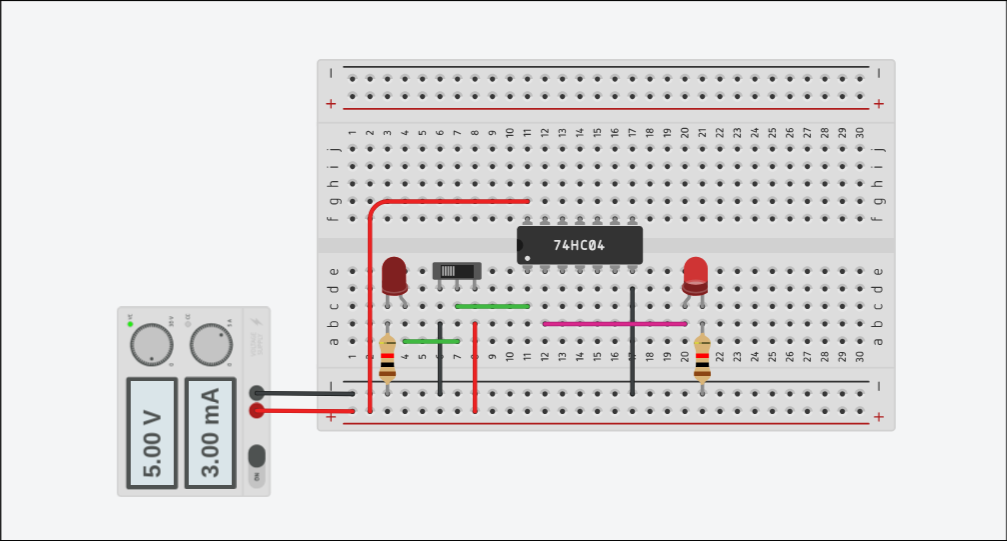
\includegraphics[width=\textwidth]{tc_exp1_off.png}
        \caption*{(a) Switch OFF (Output HIGH)}
    \end{minipage}
    \hfill
    \begin{minipage}{0.48\textwidth}
        \centering
        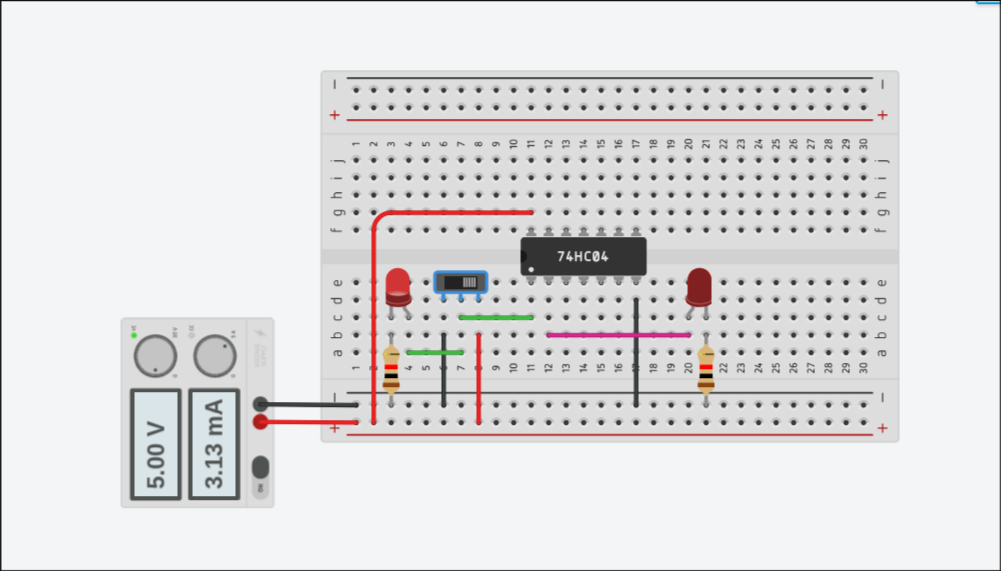
\includegraphics[width=\textwidth]{tc_exp1_on.png}
        \caption*{(b) Switch ON (Output LOW)}
    \end{minipage}
    \caption{Tinkercad Simulation Screenshot}
    \label{fig:exp1_tc}
\end{figure}

\subsection{Hardware Setup Photograph}
\begin{figure}[H]
    \begin{minipage}{0.48\textwidth}
        \centering
        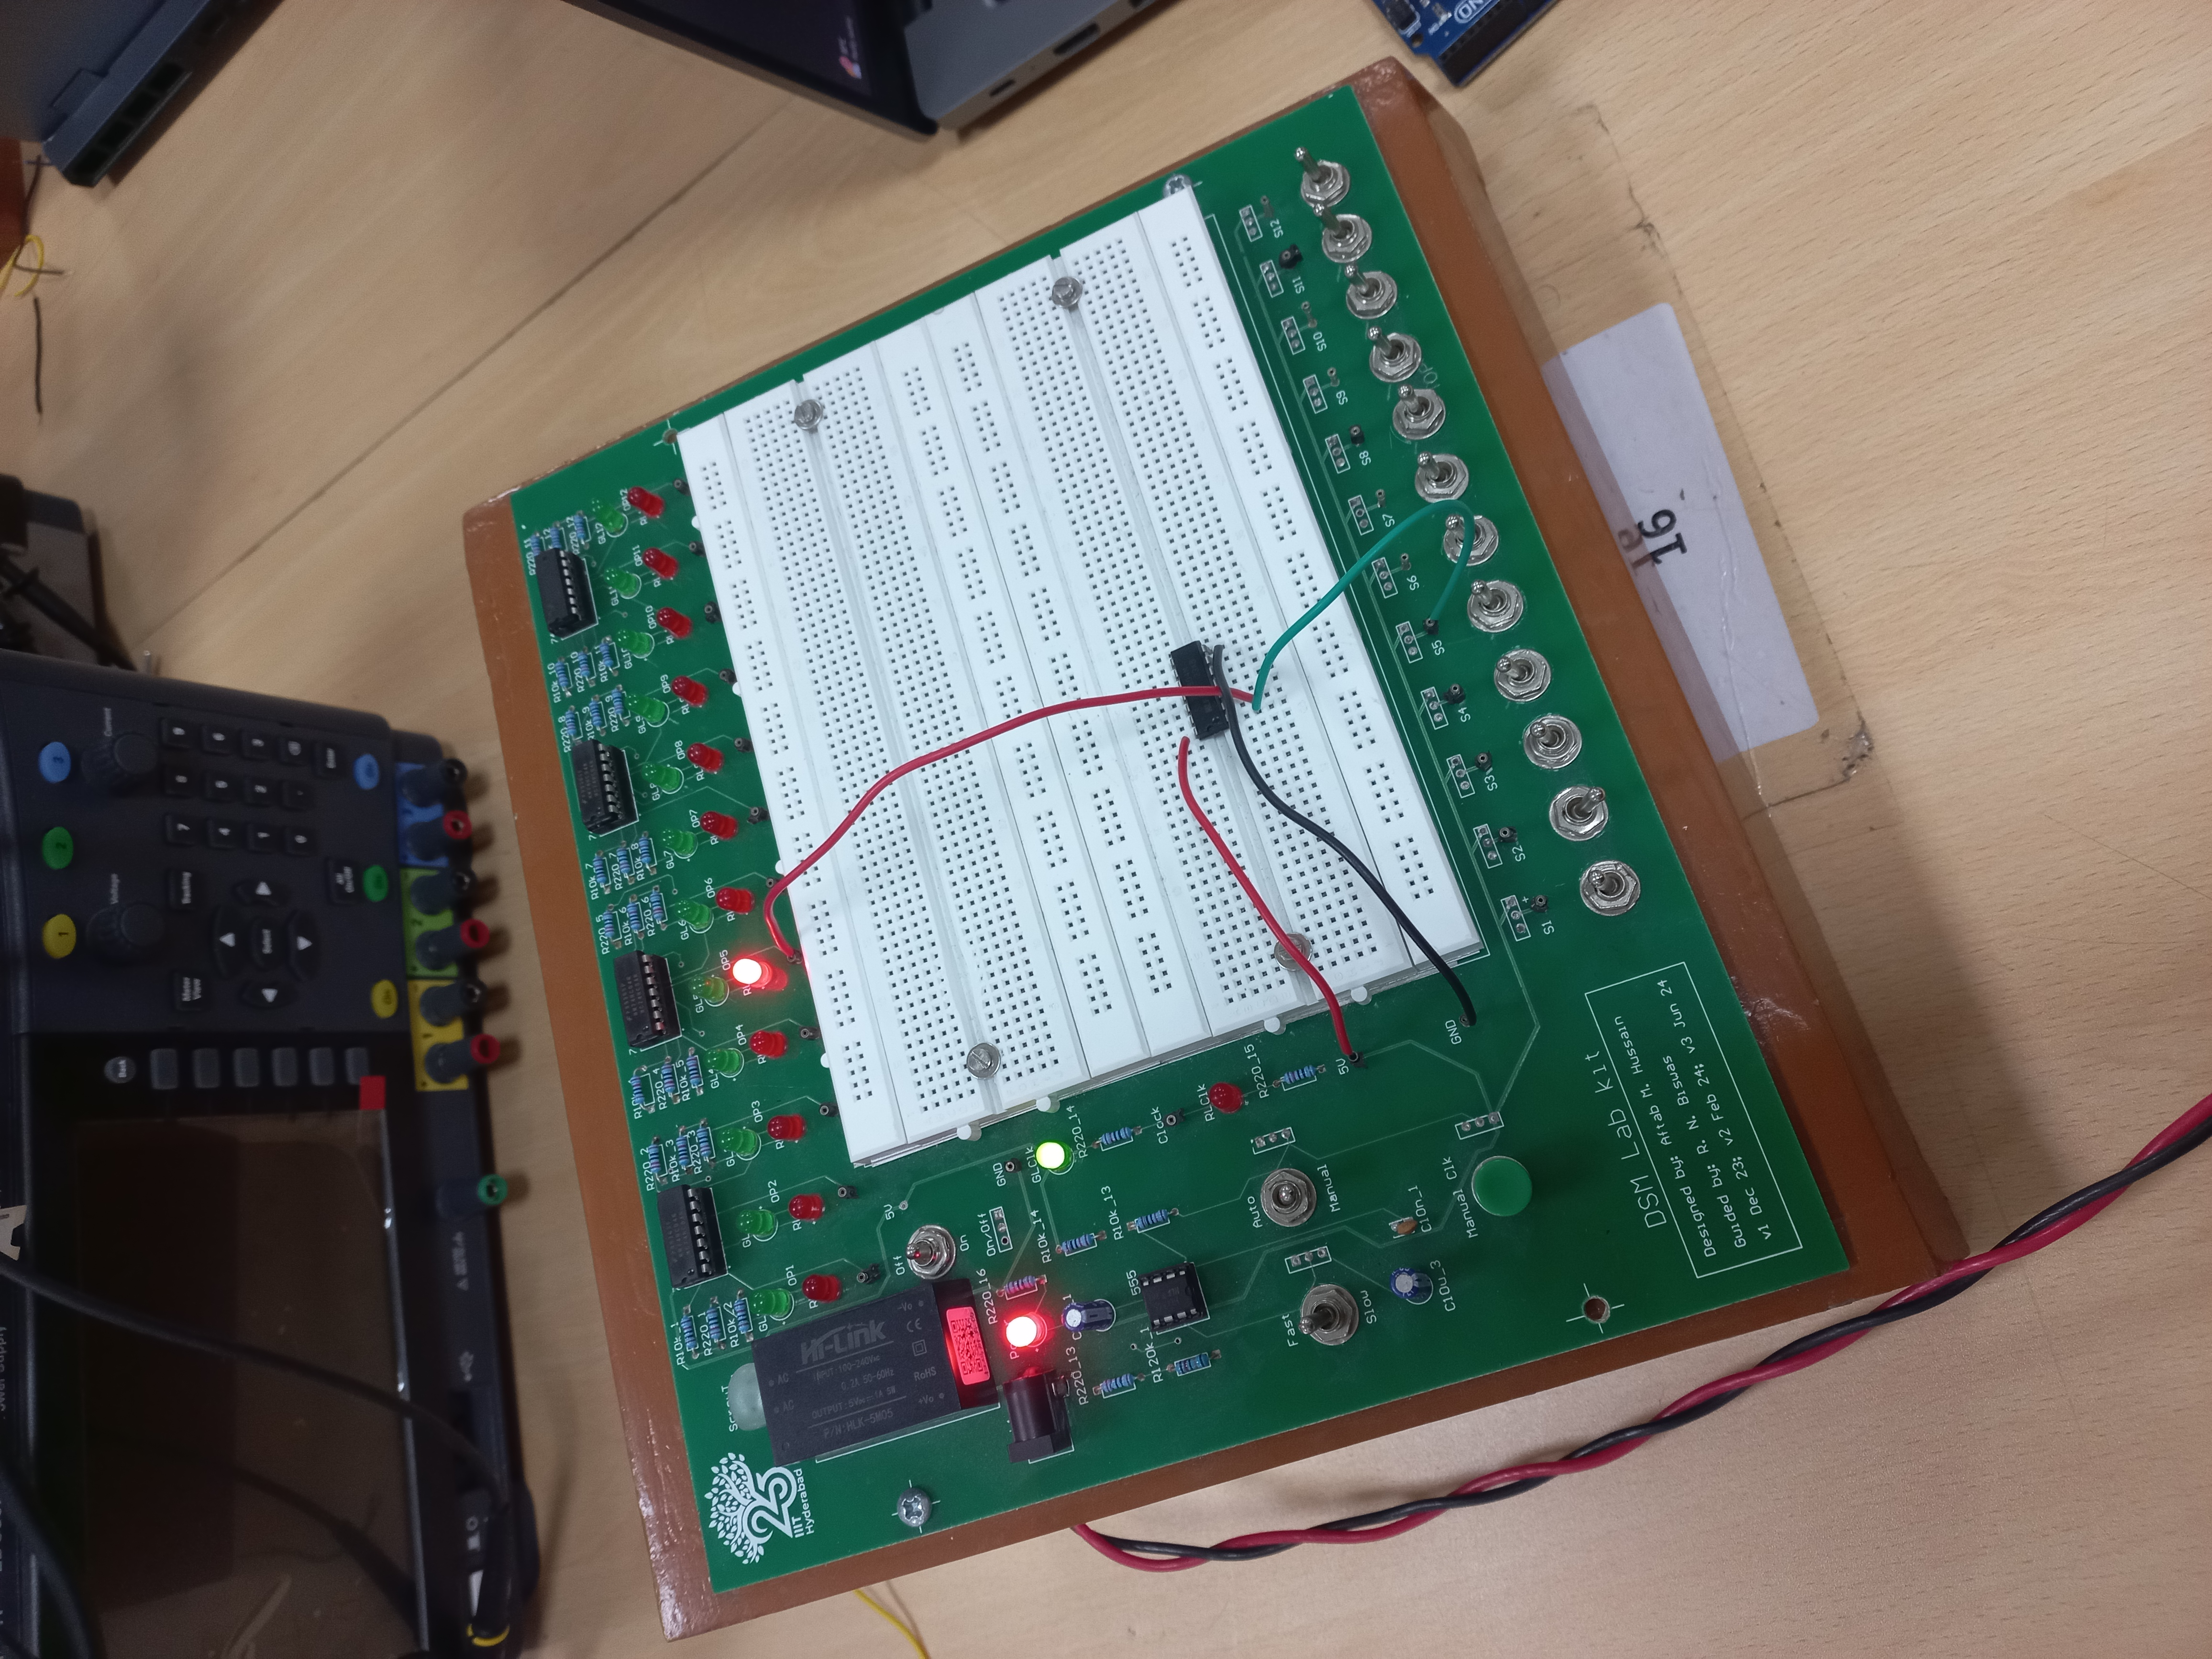
\includegraphics[width=\textwidth, angle=-90]{lab_exp1_off.jpg}
        \caption*{(a) Switch OFF (Output HIGH / Green LED)}
    \end{minipage}
    \hfill
    \begin{minipage}{0.48\textwidth}
        \centering
        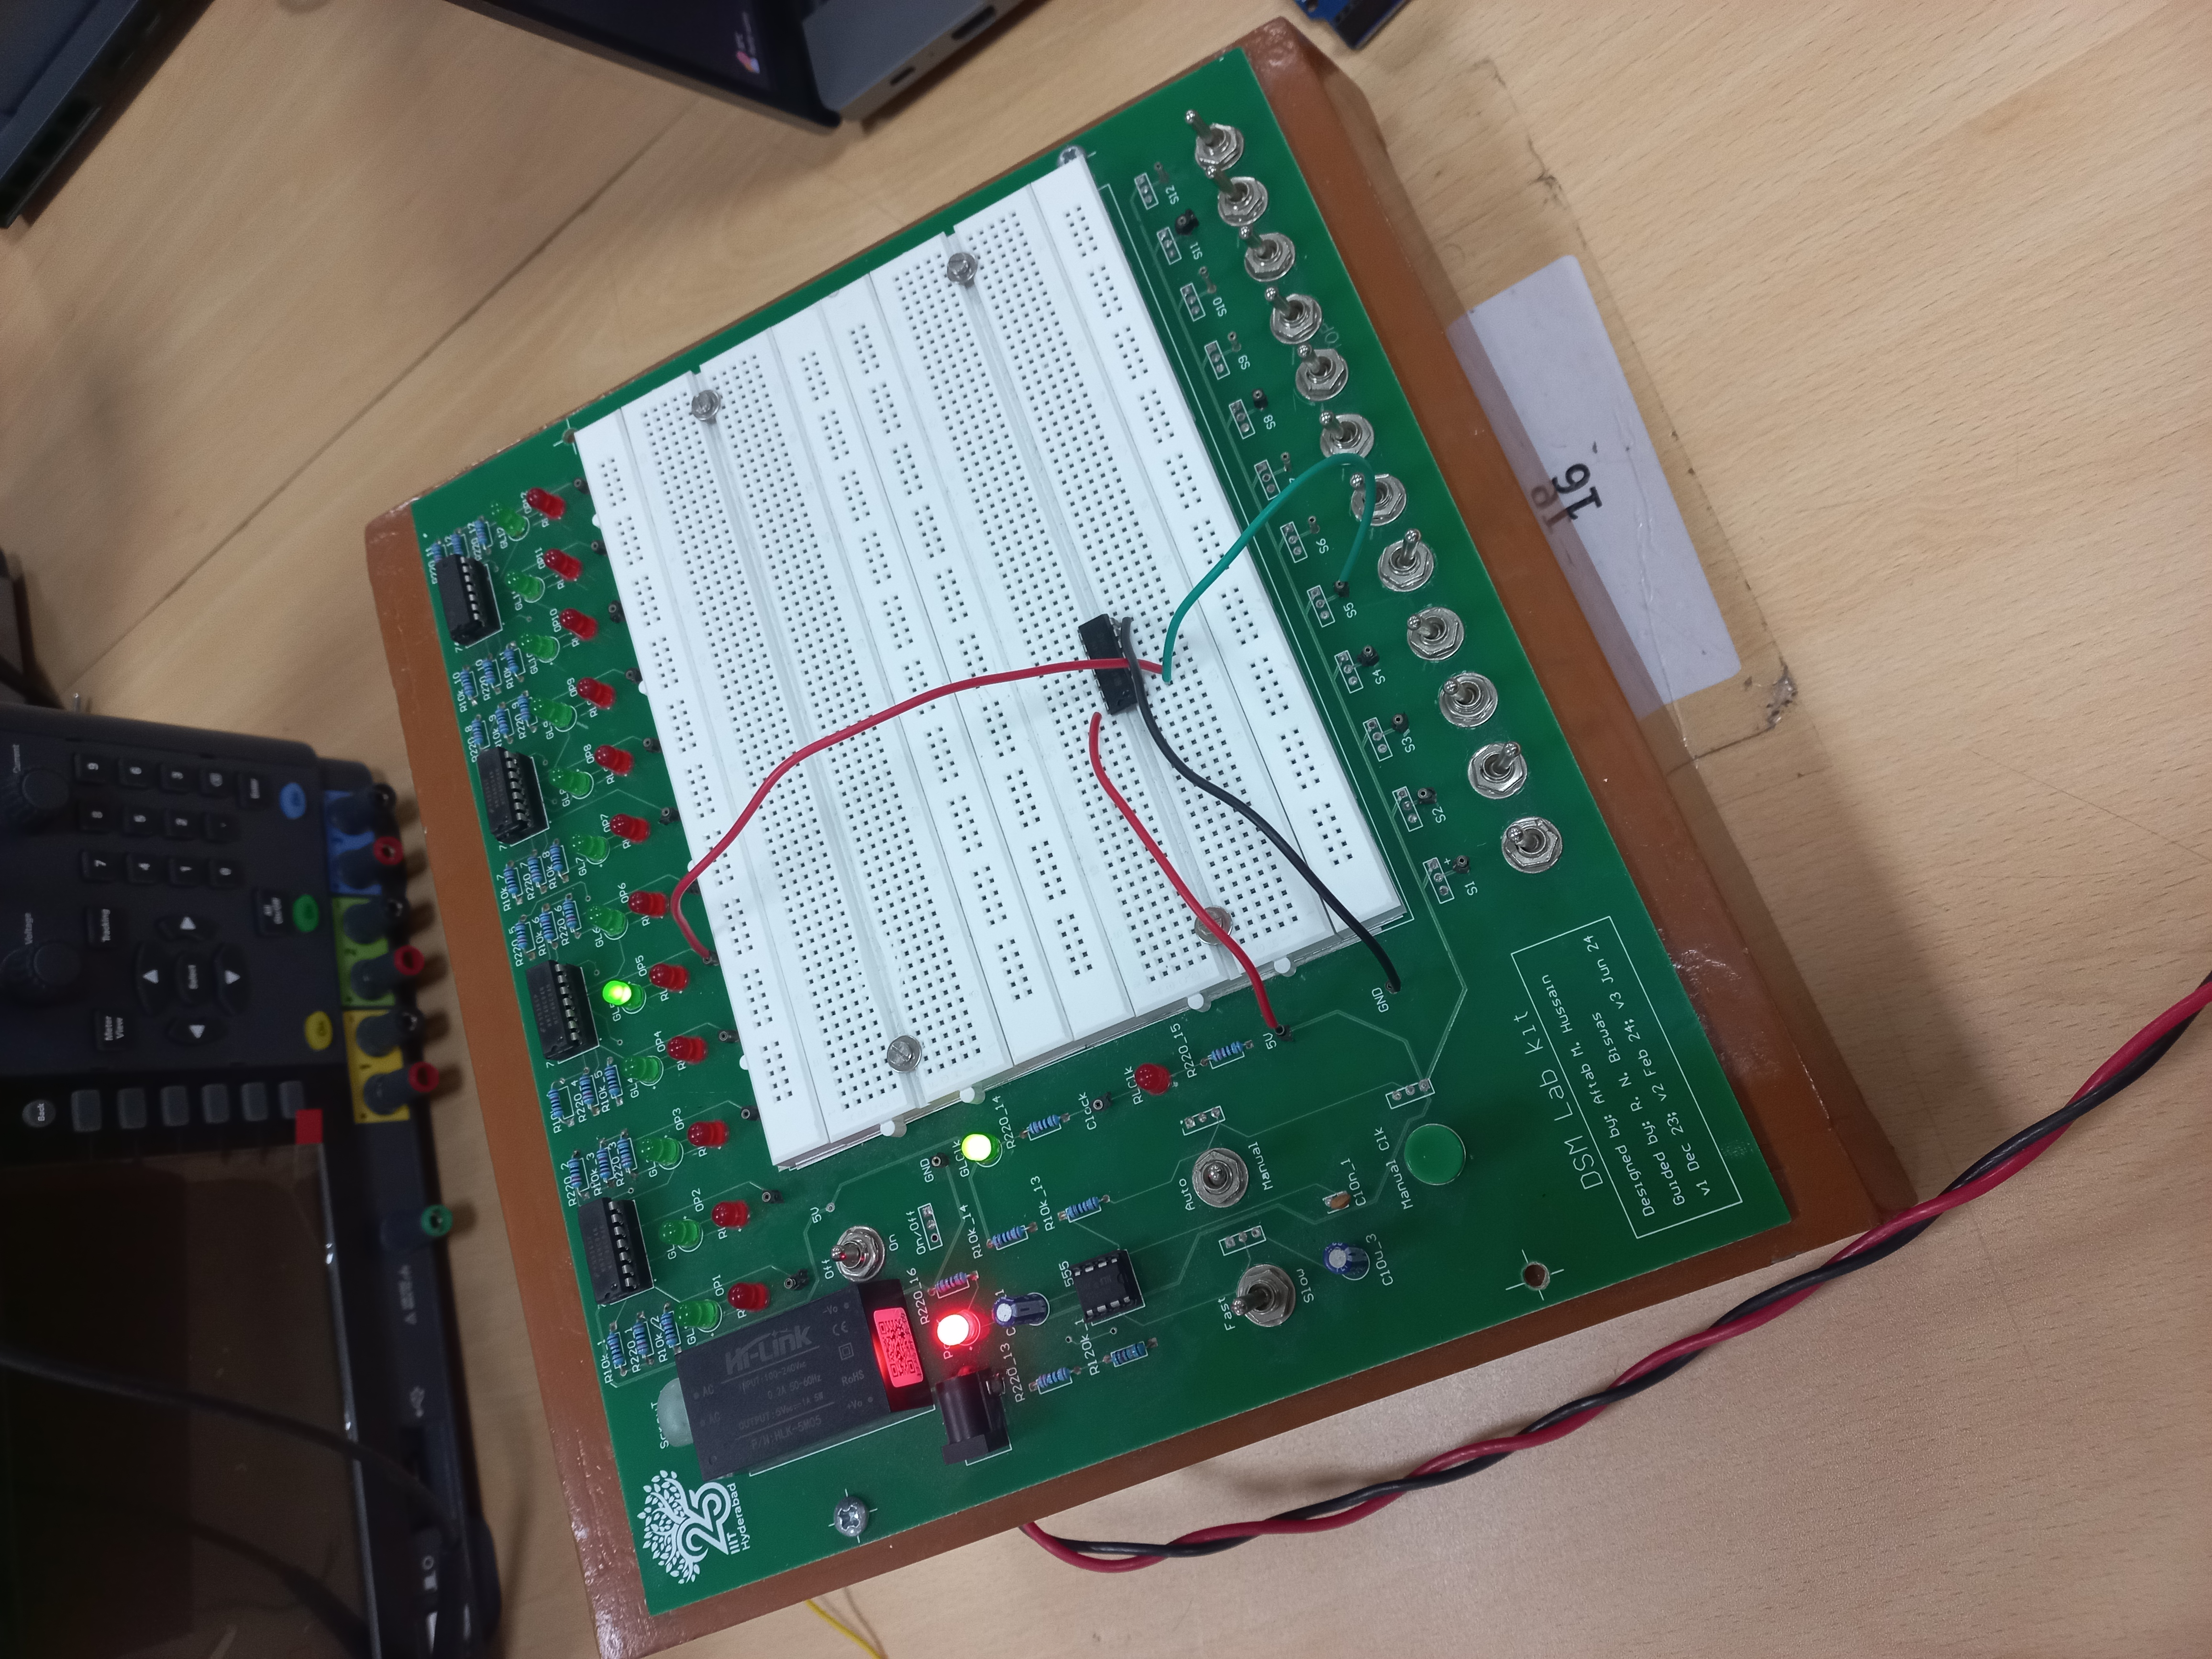
\includegraphics[width=\textwidth, angle=-90]{lab_exp1_on.jpg}
        \caption*{(b) Switch ON (Output LOW / Green LED)}
    \end{minipage}
    \caption{Hardware Setup}
    \label{fig:exp1_setup_photo}
\end{figure}

\subsection{Conclusion}
\begin{itemize}
    \item \textbf{Digital Test Kit Functional Verification}
    \item \textbf{IC 7404 Operation:} The IC 7404 TTL Hex Inverter behaved according to boolean logic rules ($Y = \bar{A}$) as expected.
    \item \textbf{Experimental Validation:} The experimental observations matched the theoretical truth table of NOT gate.
\end{itemize}

\newpage

% ==============================================================================
% experiment 2
% ==============================================================================

\section{Experiment 2}

\subsection{Aim}
\begin{itemize}
    \item Learn how to write and compile code for ATmega328P microcontroller in Arduino.
    \item Write a program output "ON" and "OFF" to serial monitor based on output of NOT gate.
\end{itemize}

\subsection{Components \& Equipment Required}
\begin{itemize}
    \item Digital Test Kit (includes power supply, switches, LEDs and breadboard)
    \item IC 7404 (TTL hex inverter)
    \item Connecting Wires
    \item Arduino Uno
    \item USB A-to-B cable
\end{itemize}

% \subsection{Hypothesis \& Reference Circuit}
% TBDl
% \begin{figure}[H]
%     \centering
%     % \includegraphics[width=0.6\textwidth]{path_to_reference_circuit_exp2.png}
%     \caption{Reference Circuit Schematic for Experiment 2}
%     \label{fig:exp2_circuit}
% \end{figure}

\subsection{Procedure}
\begin{enumerate}
    \item \textbf{Hardware Setup:}
    \begin{enumerate}
        \item Retain the IC 7404 setup on the breadboard from Experiment 1.
        \item Connect a common ground wire between the ground rail ($\text{GND}$) of the Digital Test Kit and a $\text{GND}$ pin on the Arduino Uno to ensure a unified logic reference level.
        \item Tap the output signal of the inverter using a jumper wire and connect it directly to a digital input pin on the Arduino Uno board.
    \end{enumerate}

    \item \textbf{Software:}
    \begin{enumerate}
        \item Download and install the Arduino IDE.
        \item Connect the Arduino Uno to the computer via a USB A-to-B cable.
        \item Write the code to continuously read the digital voltage level using \texttt{digitalRead()} and output the corresponding logic state to the Serial Monitor.
        \item Select the correct board (\textit{Arduino Uno}) and Serial Port under the \textbf{Tools} menu. Then compile and upload the sketch to the microcontroller.
    \end{enumerate}

    \item \textbf{Observation:}
    \begin{enumerate}
        \item Open the \textit{Serial Monitor} inside the Arduino IDE.
        \item Toggle the physical switch between LOW and HIGH logic levels.
        \item Simultaneously observe and cross-verify:
        \begin{itemize}
            \item The position of the input toggle switch.
            \item The active state of the dual-color indicator LED.
            \item The printed logic state on the Arduino IDE Serial Monitor.
        \end{itemize}
        \item Verify that the state logged on the Serial Monitor matches the inverted logic output displayed by the indicator LED.
    \end{enumerate}
\end{enumerate}

\subsection{Arduino Code}
\begin{lstlisting}[language=C++, caption={Arduino Code for Experiment 2}]
#define IN_PIN 8

void setup() {
  Serial.begin(9600);
  pinMode(IN_PIN, INPUT);
}

void loop() {
  int val = digitalRead(IN_PIN);
  
  if (val == HIGH) Serial.println("ON");
  else Serial.println("OFF");
  
  delay(500);
}
\end{lstlisting}

\subsection{Observations}
\begin{table}[H]
    \centering
    \caption{Observations for Experiment 2}

    \vspace{0.2cm}
    
    \begin{tabular}{ccc}
        \toprule
        \textbf{Switch} & \textbf{Indicator LED} & \textbf{Serial Monitor Output} \\
        \midrule
        OFF & Red (Logic 1) & ON \\
        ON & Green (Logic 0) & OFF \\
        \bottomrule
    \end{tabular}
\end{table}

\subsection{Tinkercad Simulation}
\noindent \textbf{Tinkercad Link:} \href{https://www.tinkercad.com/things/8qwsLC6OCPk-dsm-lab-1-exp-2?sharecode=xAkWi6HZX8T_sagvYBEkhLrVyf_oJyhEkiC-yYp4X4U}{\color{blue}Click here}
\begin{figure}[H]
\centering
    \begin{minipage}{0.48\textwidth}
        \centering
        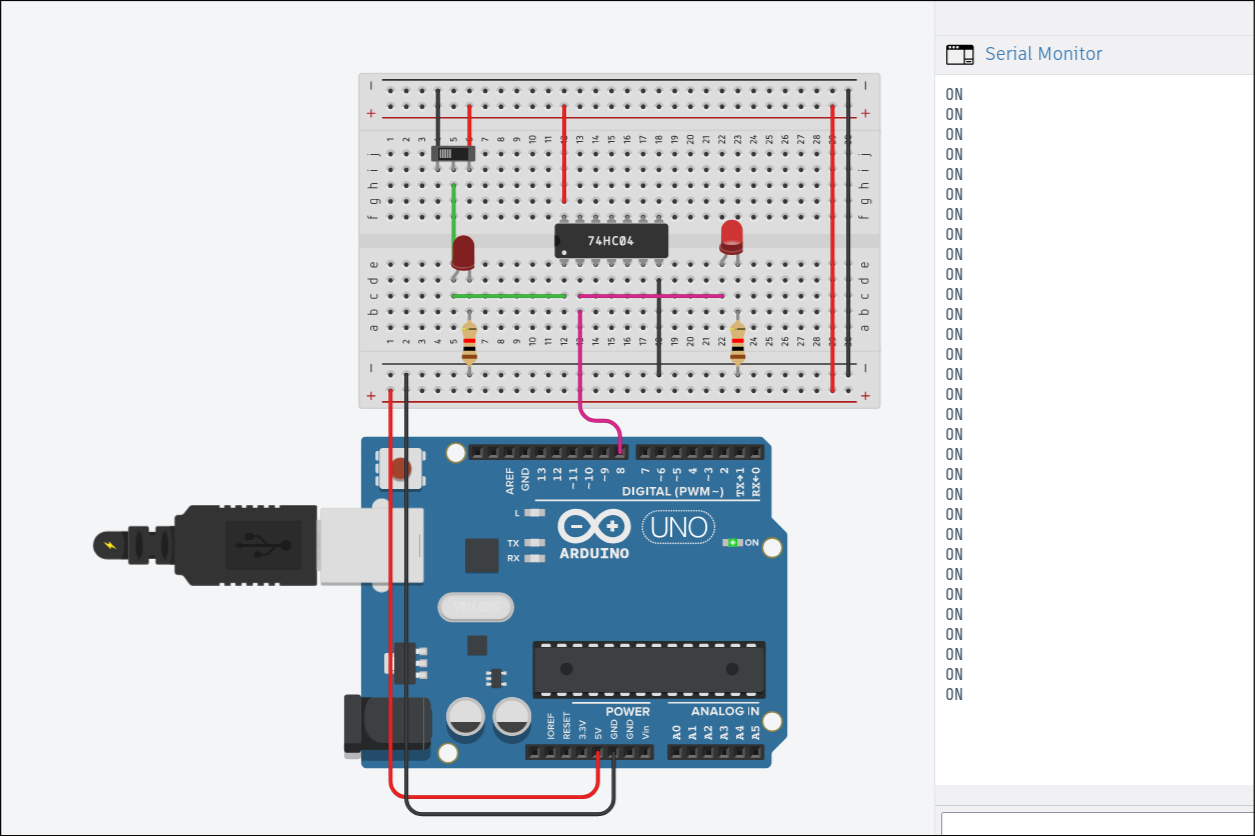
\includegraphics[width=\textwidth]{tc_exp2_off.png}
        \caption*{(a) Switch OFF}
    \end{minipage}
    \hfill
    \begin{minipage}{0.48\textwidth}
        \centering
        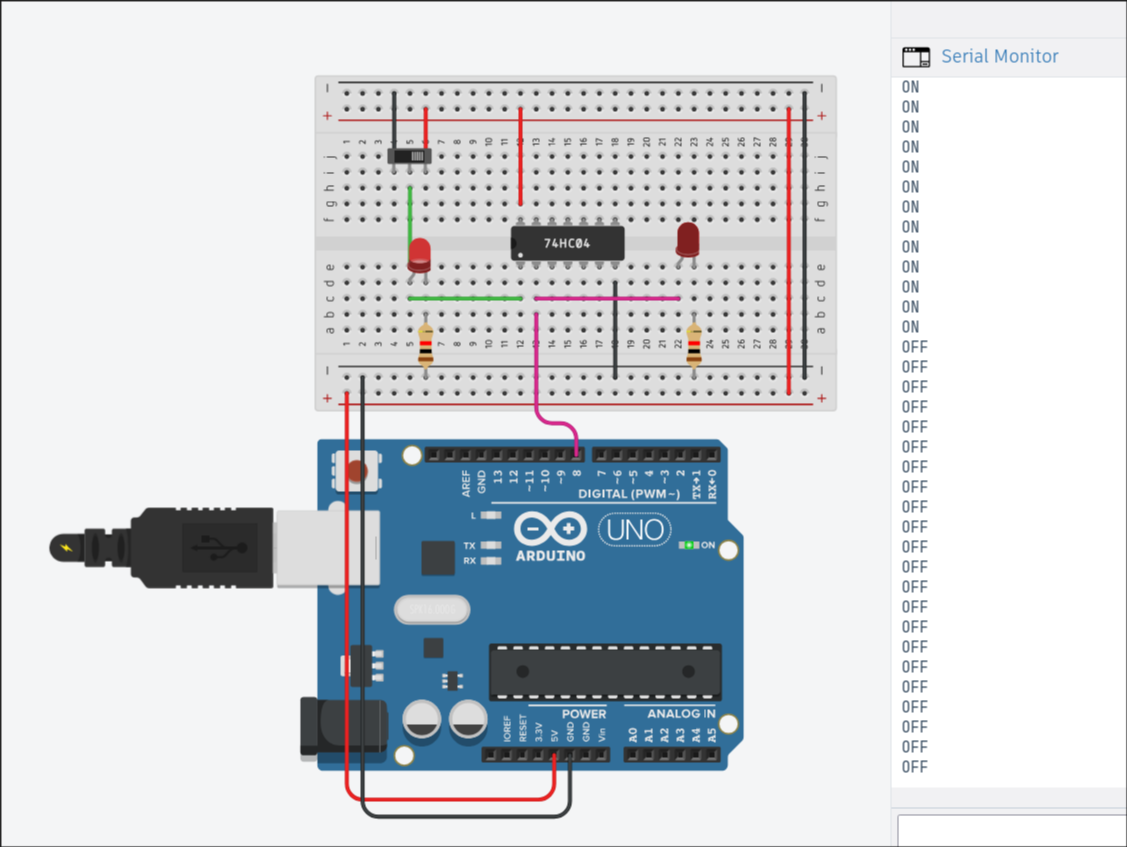
\includegraphics[width=\textwidth]{tc_exp2_on.png}
        \caption*{(b) Switch ON}
    \end{minipage}
    \caption{Tinkercad Simulation Screenshot}
    \label{fig:exp2_tc}
\end{figure}

\subsection{Hardware Setup Photograph}
\begin{figure}[H]
    \begin{minipage}{0.48\textwidth}
        \centering
        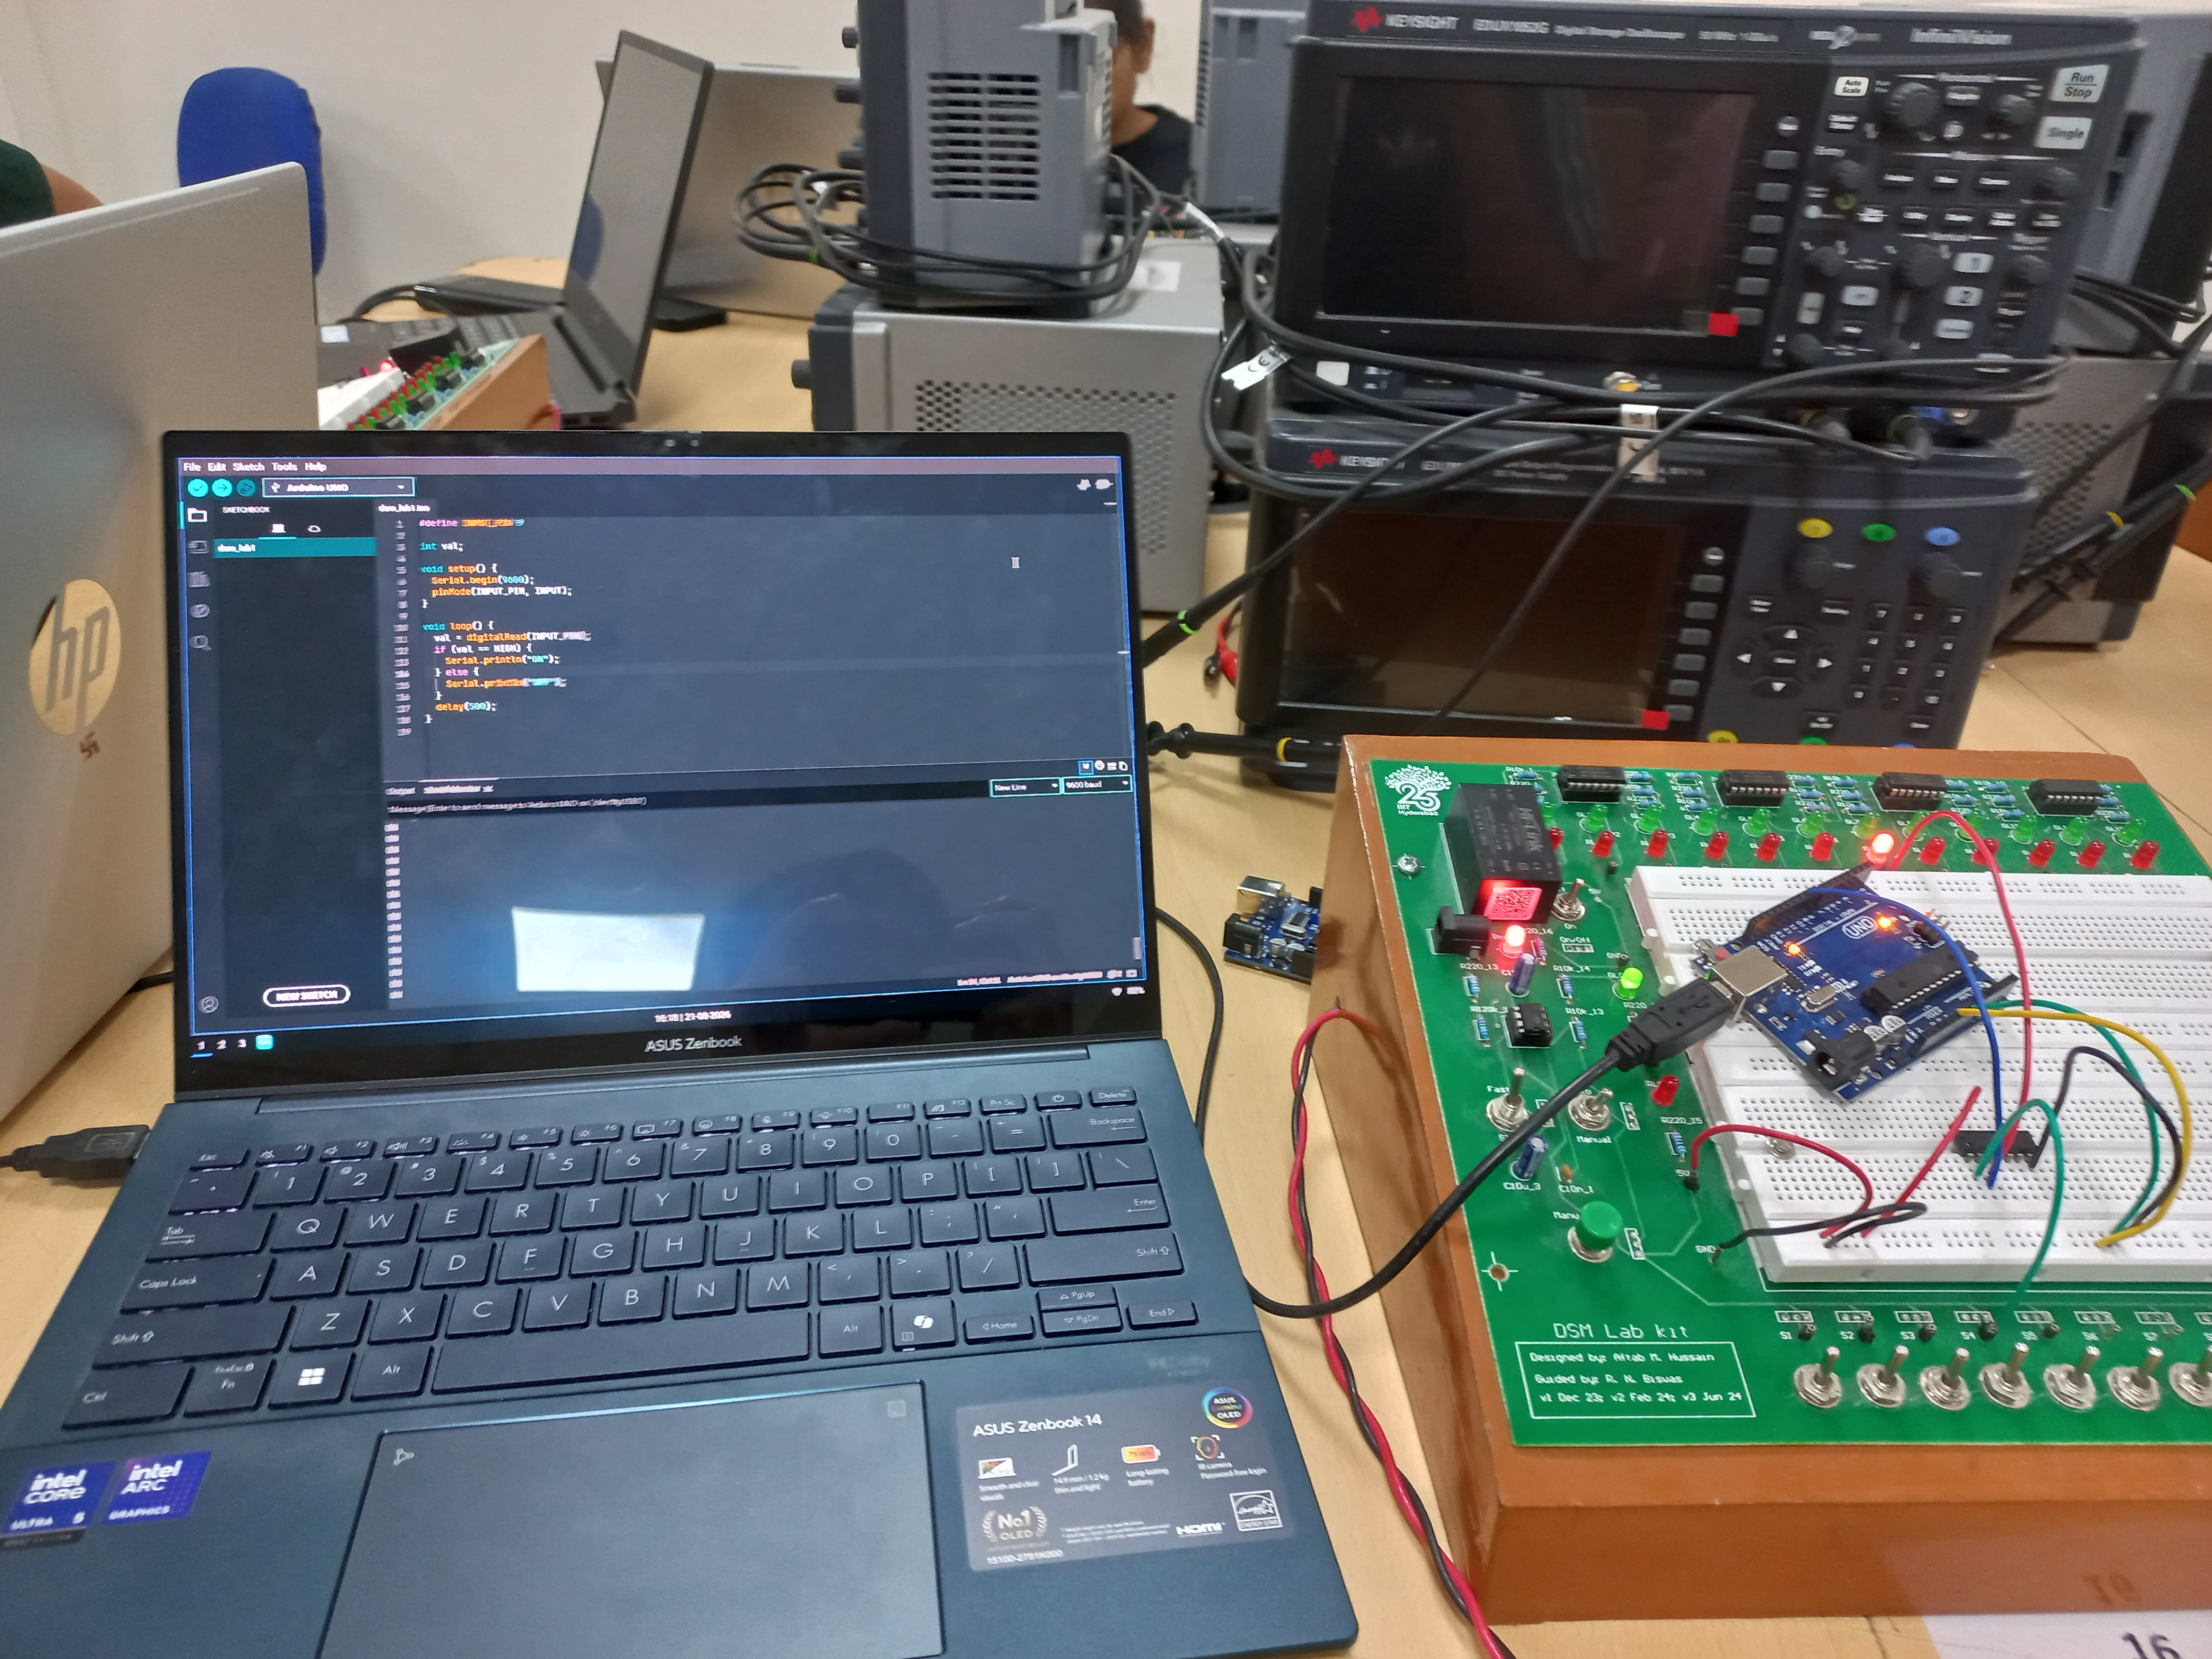
\includegraphics[width=\textwidth]{lab_exp2_off.jpg}
        \caption*{(a) Switch OFF}
    \end{minipage}
    \hfill
    \begin{minipage}{0.48\textwidth}
        \centering
        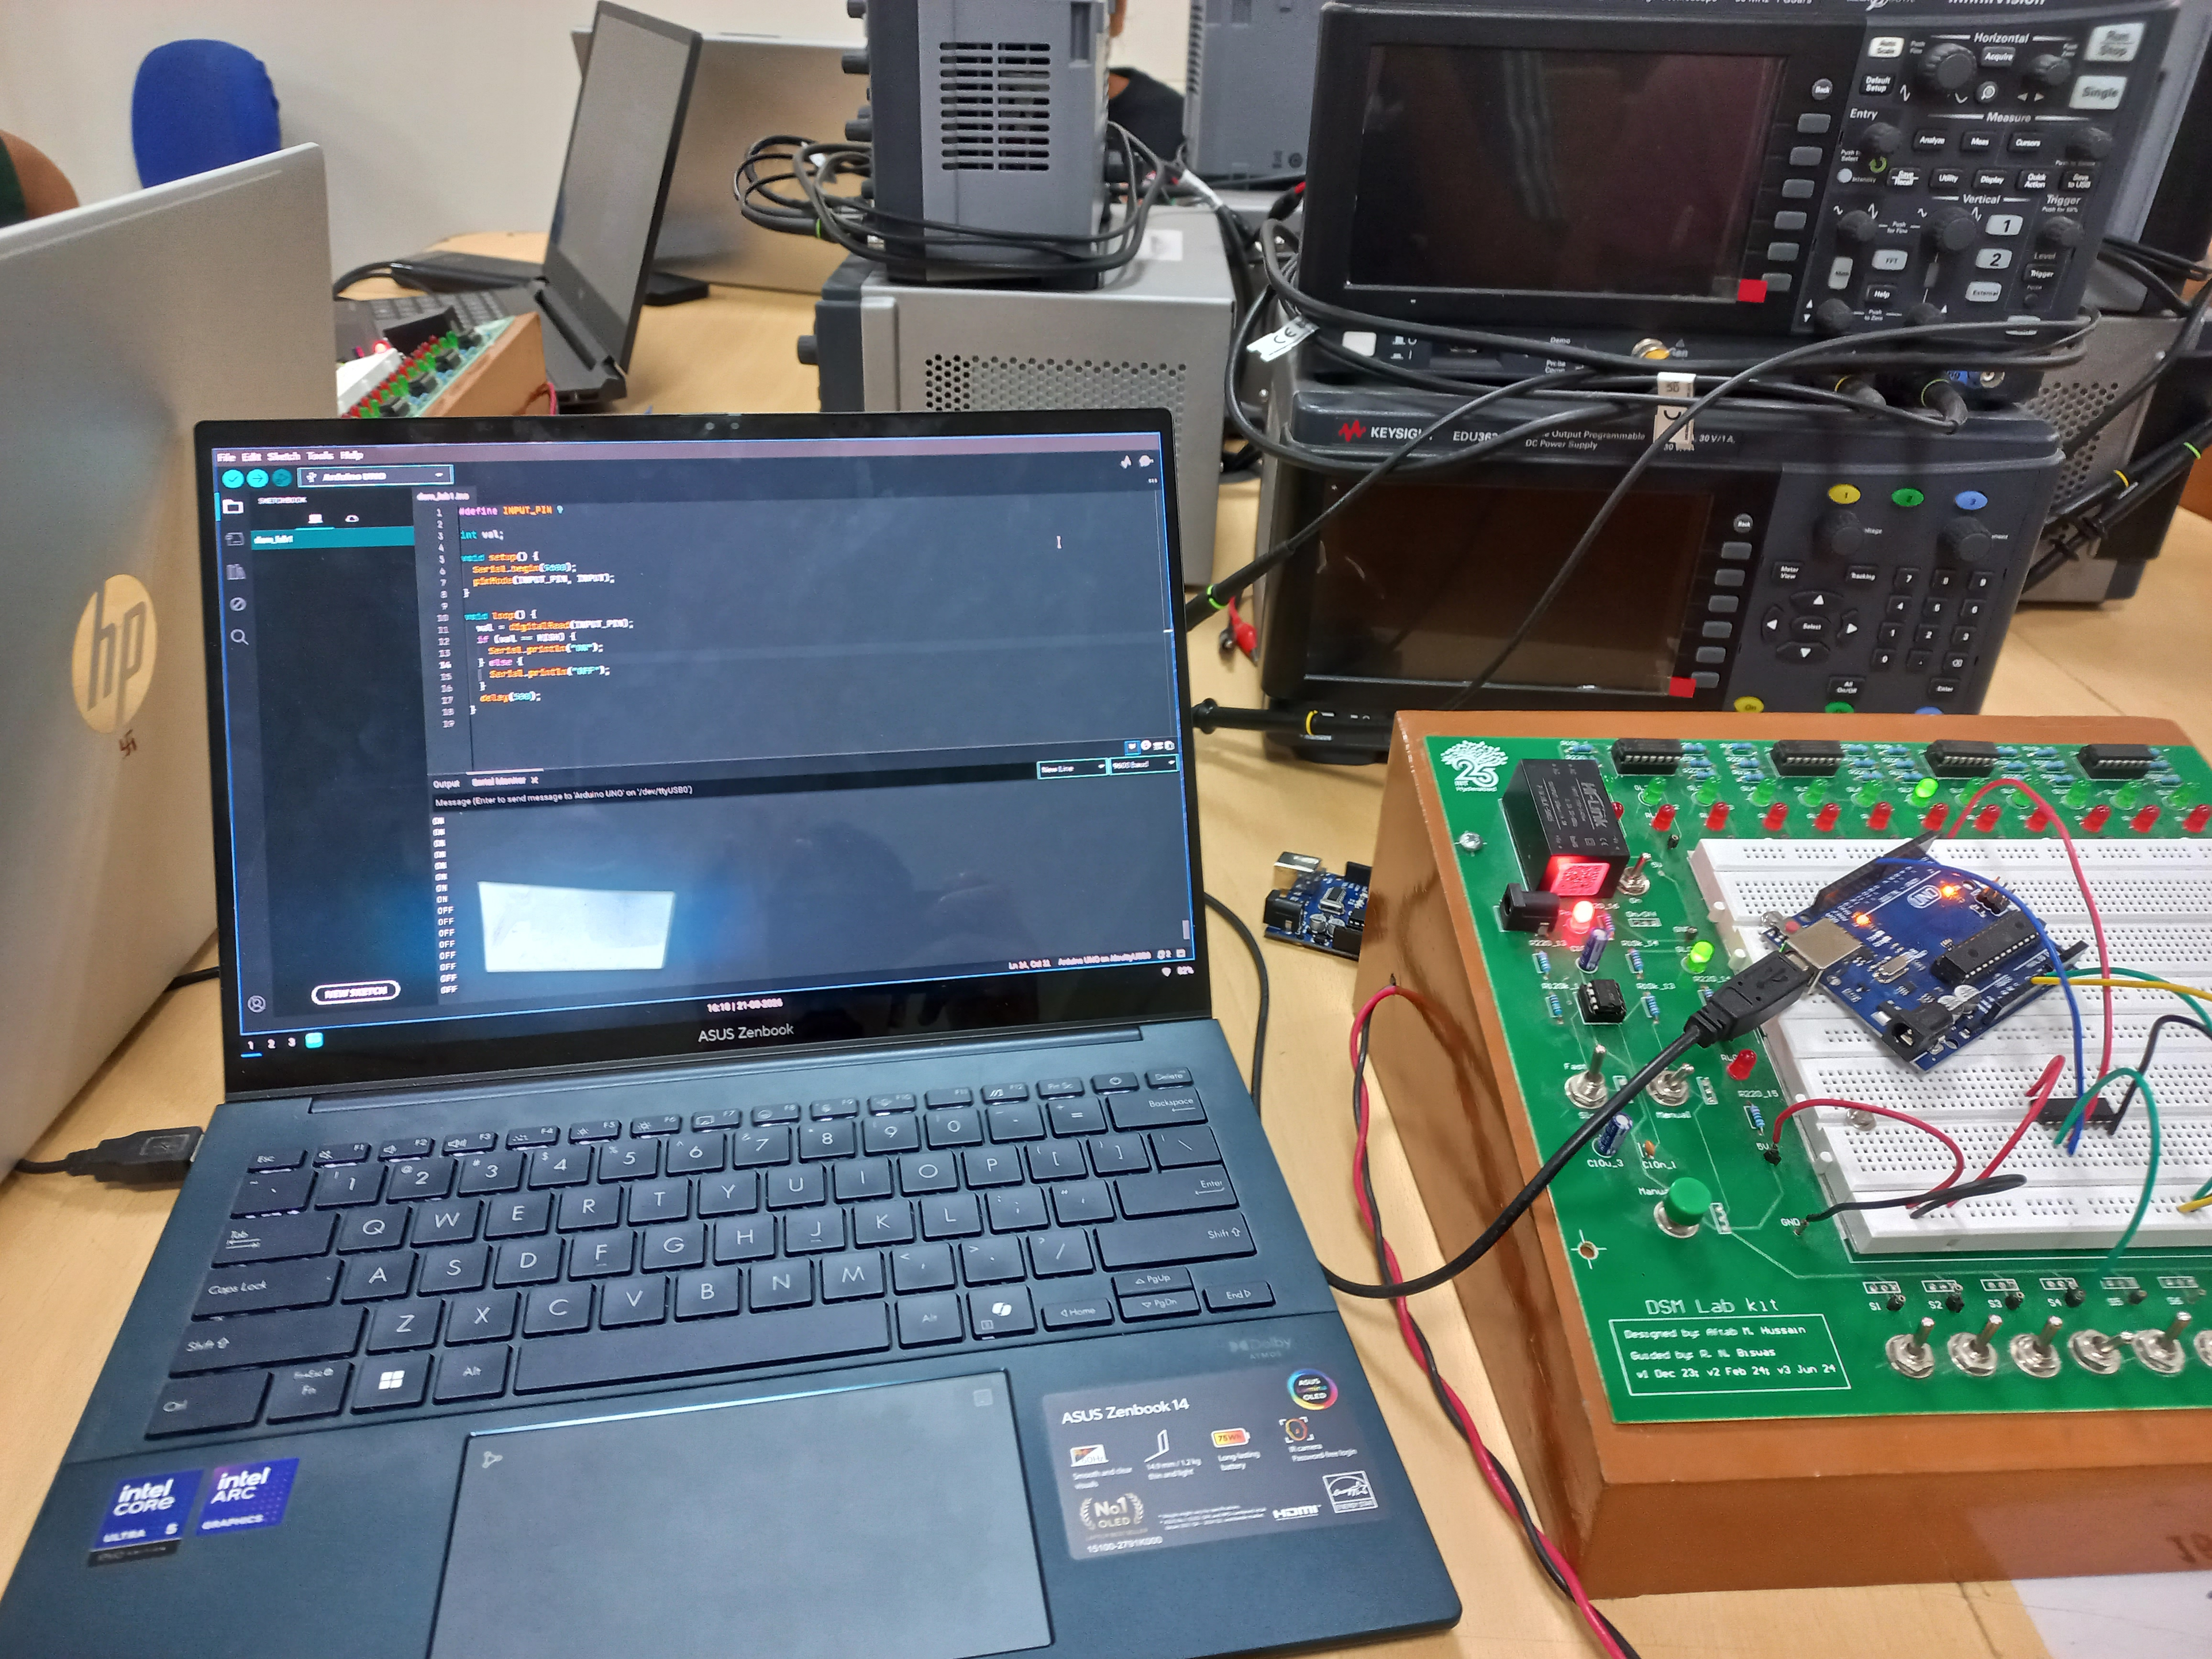
\includegraphics[width=\textwidth]{lab_exp2_on.jpg}
        \caption*{(b) Switch ON}
    \end{minipage}
    \caption{Hardware Setup}
    \label{fig:exp2_setup_photo}
\end{figure}

\subsection{Conclusion}
We successfully configured the software environment to write, compile, and upload C++ code to the Arduino Uno. The real-time readings captured on the Serial Monitor matched with the physical LED indicators and input switch states.

\end{document}